% This document must be compiled with XeLatex
\documentclass[10pt, a4paper]{article}

\usepackage{polyglossia}
\usepackage{fontspec}
\usepackage{graphicx}
\usepackage{float}
\usepackage{xcolor}
\usepackage{hyperref}
\usepackage{listings}
\usepackage{setspace}
\usepackage{tcolorbox}

% Config to language and sangria
\setdefaultlanguage{spanish}

% Config to code block
\lstset {
  frame=tb,
  backgroundcolor=\color{white},
  numbers=none,
  numberstyle=\tiny,
  breaklines=true,
  basicstyle=\ttfamily\footnotesize,
  keywordstyle=\color{blue},
  commentstyle=\color{green!50!black},
}

\begin{document}

\section{Introducción: Investigación
operativa}\label{sec:introduction-operations-research}

Scheduling (programación de tareas). Consiste en asignar recursos a actividades en
el tiempo. Matematicamente estos problemas estan calificados como los más 
dificiles

\subsection{Flow Shop Scheduling Problem
(FSSP)}\label{sec:flow-shop-scheduling-problem-fssp}

Es un problema de lineas de producción. Los trabajos $J_i$ deben ser procesados 
en las máquinas $M_i$ con tiempos fijos $p_{ji}$ y son independientes para cada 
trabajo. Además asumimos que los tiempos de trabajo ya han sido optimizados.

\begin{figure}[H]
  \centering
  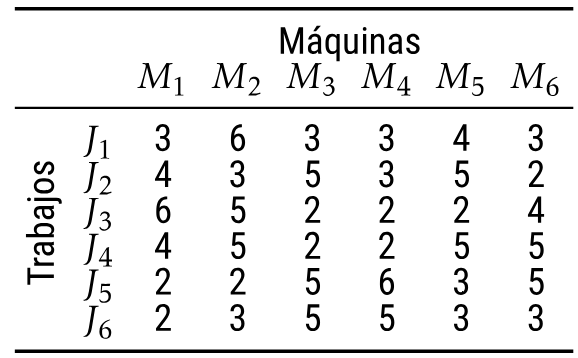
\includegraphics[width=0.5\textwidth]{./.github/1733238439.png}
  \caption{Instancia a analizar}\label{fig:instance-of-analysis}
\end{figure}

Rápidamente, sin analizar el tiempo que puede demorar encontrar la solución 
optima; podemos pensar en diseñar un algoritmo de fuerza bruta, es sencillo 
para nosotros pero imposible para la máquina.

\begin{figure}[H]
  \centering
  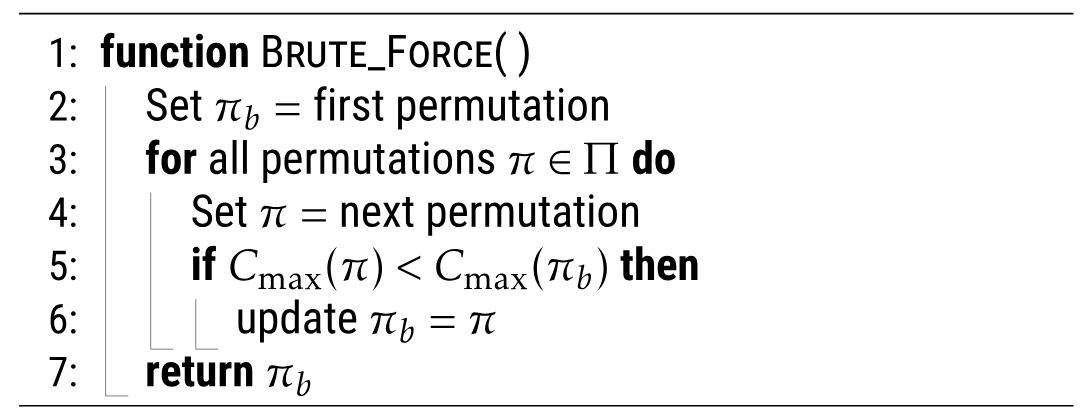
\includegraphics[width=0.8\textwidth]{./.github/1733239898.png}
  \caption{Algoritmo de fuerza bruta}\label{fig:brute-force-algoritm}
\end{figure}

\subsection{¿Qué es una Heurística?}

Procedimiento simple diseñado de manera inteligente para crear una solución o 
para buscar mejores soluciones que satisfagan a cierto problema de optimización.

\begin{itemize}
  \item Idea, criterio, método, o regla que ayuda a decidir cuál alternativa 
    es mejor
  \item Idea basada en la intuición o en el sentido común
  \item Idea que utiliza la estructura o contexto del problema
\end{itemize}

La primera Heurística en la historia fue nombrada \textit{Método Monte Carlo} y se 
basaba en escoger una muestra del total y observar cuántos cumplen con el propósito.

\subsubsection{Búsqueda aleatoria para el FSSP}

Selecciona una muestra aleatoria extraída del espacio de soluciones para encontrar
un resultado númerico (media esperada, mejor, peor)

\begin{figure}[H]
  \centering
  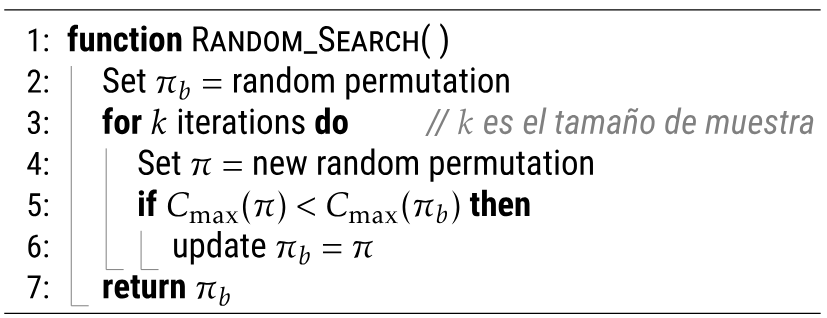
\includegraphics[width=0.8\textwidth]{./.github/1733241212.png}
  \caption{Búsqueda aleatoria}\label{fig:random-search}
\end{figure}

Este enfoque es muy general y puede ayudar a resolver otro tipo de problemas. Sin
embargo, no es el mejor para resolver el problema propuesto:

\begin{itemize}
  \item La muestra puede ser demasiado pequeña y no representativa
  \item La media de la muestra $\approx$ la media de la población
  \item El mejor de la muestra no es el mejor de la población
\end{itemize}

\section{Métodos heurísticos básicos}\label{sec:basic-heuristic-methods}

\subsection{Heurísticas constructivas}\label{sec:constructive-heuristics}

Construyen una solución desde cero, añadiendo uno a uno los componentes a la 
solución parcial, hasta que la solución esté completa. La pregunta importante 
para diseñar esta Heurística es \textcolor{blue}{¿Cuál elemento 
debería añadir y cómo?}

\subsubsection{Heurística constructiva de Nawaz, Enscore y Ham}

Propuesta en $1983$ para resolver el FSSP y se divide en dos partes importantes.

\paragraph{Primera etapa: \textcolor{blue}{Cuál es el elemento que debo insertar}}

Determina un orden de inserción. En este caso, se ordena del más 
grande al más pequeño según su tiempo total de procesamiento.
$\pi_0 = (J_4, J_5, J_1, J_2, J_3, J_6)$

\paragraph{Segunda etapa: \textcolor{blue}{Cómo o dónde lo debo de insertar}}

Insertar estos trabajos, uno a uno, en la mejor posición, comenzando con 
$\pi = (J_4)$

\begin{figure}[H]
  \centering
  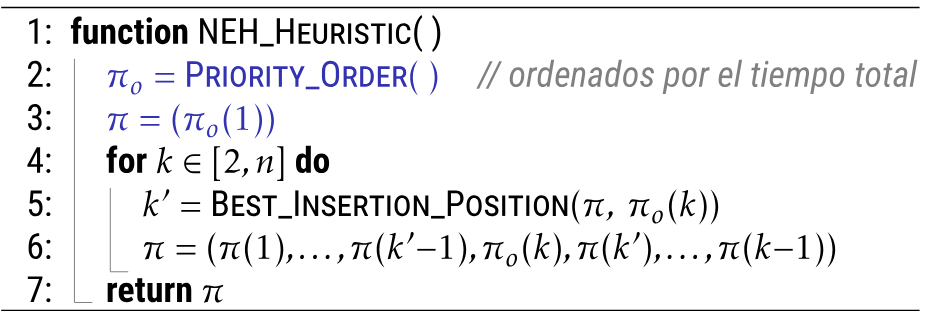
\includegraphics[width=0.8\textwidth]{./.github/1733245449.png}
  \caption{Heurística NEH}\label{fig:NEH-heuristic}
\end{figure}

\begin{itemize}
  \item Si ocurre empates al realizar la segunda etapa, se ha probado que existe
    una técnia para solucionar este problema, por el momento solo cogemos el 
    orden del primer resultado.

  \item La calidad de la solución se mide con el desvío relativo
    \[
      DR = \frac{C_{\max}(\pi) - C_{\max}(\pi^*)}{C_{\max}(\pi^*)}
    \]
\end{itemize}

\subsubsection{Costo de la Heurística constructiva}
Tenemos que analizar los costos en las dos partes que componen el algoritmo.

\begin{itemize}
  \item Ordenar cuesta $O(nlogn)$

  \item NEH evalúá $\frac{n(n+1)}{2-1}$ programas parciales, y esto es $O(n^2)$. 
    Recordemos que cuando insertamos el primer trabajo, no comparamos con nada;
    luego cuando insertamos el segundo trabajo, lo podemos insertar antes o 
    después del primer trabajo y asi sucesivamente.

  \item Finalmente, evaluar cada programa parcial significa evaluar los $J_i$ 
    trabajos en las $M_j$ máquinas. Por lo tanto el costo es $O(nm)$
\end{itemize}

\textcolor{blue}{Entonces, la Heurística constructiva NEH original tiene un tiempo 
de ejecución de $O(n^3m)$.}

\singlespacing

Sin embargo Taillard calculó la mejor posición de inserción en cuatro matrices 
de $O(nm)$. \textcolor{blue}{Con esta aceleración, NEH inserta los $n$ trabajos en 
un tiempo $O(n^2m)$}

\subsubsection{Aceleración de Taillard}

Taillard hace dos análisis para poder aplicar esta aceleración. Supongamos que 
tenemos ya programado 4 trabajos en 4 máquinas. Entonces, ¿dónde puedo agregar un 
quinto trabajo?

\paragraph{Los tiempos de finalización más tempranos}

Imaginemos que empujamos todos los trabajos hacía el inicio, lo más posible 
que se pueda. Es decir, el procesamiento del trabajo pasa a la siguiente justo 
cuando culmina su procesamiento en la primera máquina.

\textcolor{blue}{\textbf{Conclusión}: Si insertamos el quinto  trabajo en cualuquir 
lugar, nos daremos cuenta que los tiempos de finalización en cada máquina de los 
trabajos procesados antes del nuevo trabajo insertado \textbf{no cambian}}

\begin{figure}[H]
  \centering
  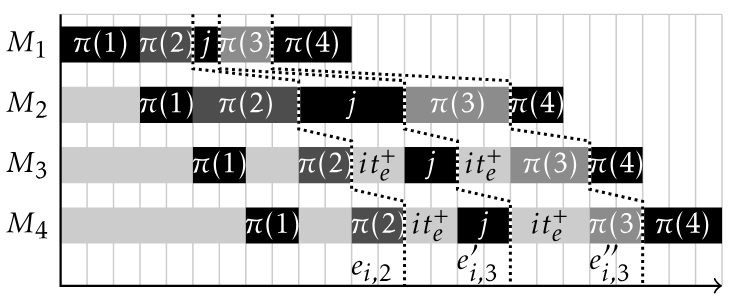
\includegraphics[width=0.8\textwidth]{./.github/1733346799.png}
  \caption{Tiempos de finalización más 
  tempranos}\label{fig:Relative-earliest-completion-times}
\end{figure}

\paragraph{Los tiempos de iniciación más tardios}

Imaginemos que empujamos los trabajos hacia el final, lo más posible 
que se pueda. Recordemos que los tiempos de procesamiento de cada trabajo en cada 
máquina varía, por lo tanto en cada máquina pueden quedar espacios sin 
procesamiento. Dichos espacios pueden ser ocupados por los trabajos que ya se 
procesaron en la máquina.

\textcolor{blue}{\textbf{Conclusión}: Si insertamos el quinto trabajo en cualquier 
lugar, nos daremos cuenta que los tiempos de iniciación tardía en cada máquina de 
los trabajos procesados después del nuevo trabajo insertado \textbf{no cambian}}

\begin{figure}[H]
  \centering
  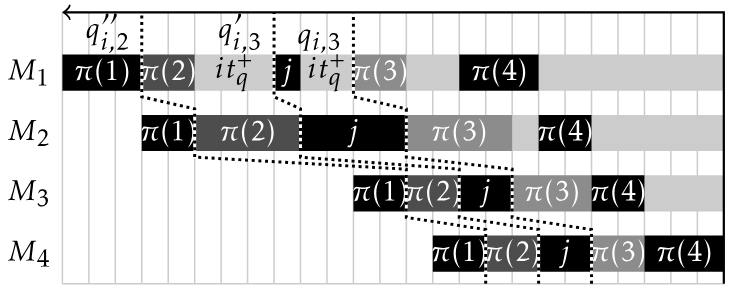
\includegraphics[width=0.8\textwidth]{./.github/1733346809.png}
  \caption{Tiempos de iniciación más 
  tardíos}\label{fig:Relative-latest-starting-times}
\end{figure}

Taillard vió que podía usarlos para calcular el \textit{Makespan}. Lo que propuso 
es realizar los siguientes cálculos para todos los trabajos en cada máquina.

\begin{enumerate}
  \item Calcular los \textbf{tiempos de finalización más tempranos}

    \[
      \pi_0 = (J_4, J_5, J_1, J_2, \textcolor{red}{J_3}, J_6) \qquad
      \pi = (J_5,J_4, J_2, J_1) \qquad  \text{Next\; work:} J_3 
    \]

    \[
      \text{Calcule}\; e_{k, i} =
      \max(e_{k, i-1},\ e_{k-1, i})+p_{\pi(k), i} \qquad
      \text{para}\; i \in [m], k \in [|\pi|] \qquad
      \text{con}\; e_{0, i} = e_{k, 0} = 0
    \]

    \begin{figure}[H]
      \centering
      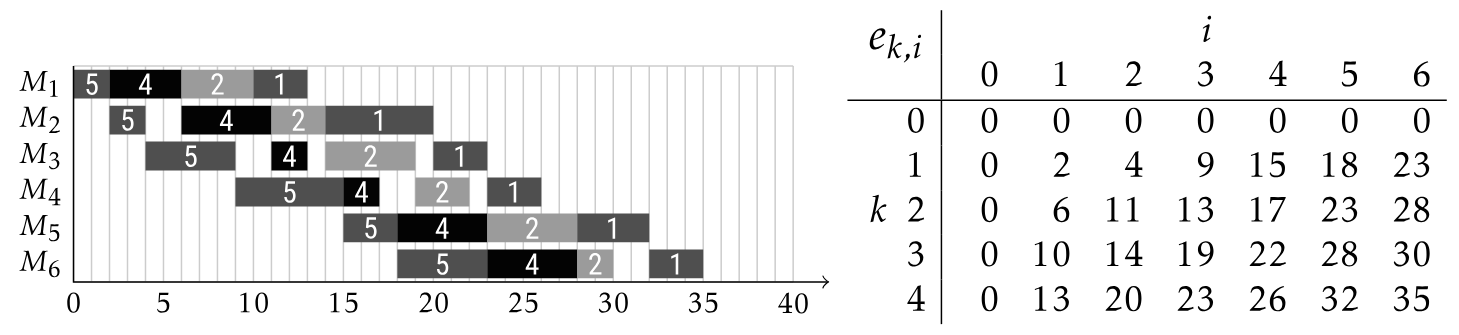
\includegraphics[width=0.8\textwidth]{
        ./.github/1733417697.png
      }
      \caption{Matriz de los tiempos de finalización más 
      tempranos}\label{fig:Relative-earliest-completion-times's-matrice}
    \end{figure}

    \textcolor{blue}{\textbf{Recuerda:} Los tiempos de finalización más 
    tempranos $e_{k, i}$ antes de la posición de inserción no cambian}

  \item calcular los tiempos de finalización con el nuevo trabajo insertado
    en cada posible posición

    \[
      \pi_0 = (J_4, J_5, J_1, J_2, \textcolor{red}{J_3}, J_6) \qquad 
      \pi = (J_5,J_4, J_2, J_1) \qquad \text{Next work:}\; J_3 
    \]

    \[
      \text{Calcule}\; e^{'}_{k, i} = 
      \max(e^{'}_{k, i-1},\ e_{k-1, i}) + p_{j, i} \qquad 
      \text{para}\; i \in [m], k \in [|\pi| + 1] \qquad 
      \text{con}\; e^{'}_{k, 0} = 0
    \]

    \begin{figure}[H]
      \centering
      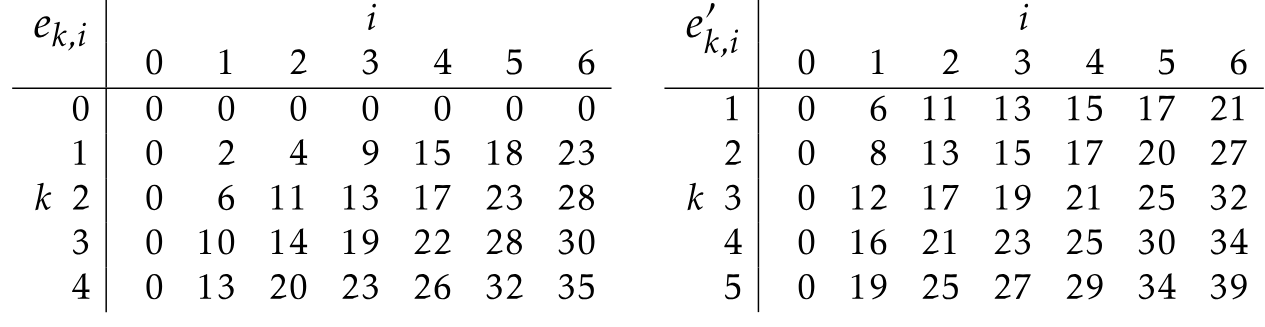
\includegraphics[width=0.8\textwidth]{
        ./.github/1733417714.png
      }
      \caption{Matriz de los tiempos de finalización más 
      tempranos más $J_3$}\label{
        fig:Relative-earliest-completion-times's-matrice-with-J3
      }
    \end{figure}

    \textcolor{blue}{Los tiempos de fin tempranos $e^{'}_{k, i}$ se calculan con 
    los tiempos $e_{k-1, i}$ y con}

    \begin{figure}[H]
      \centering
      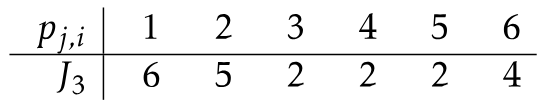
\includegraphics[width=0.4\textwidth]{
        ./.github/1733417722.png
      }
      \caption{Tiempo de proceso del 
      trabajo $J_3$}\label{fig:work_3's-process-time}
    \end{figure}

  \item Calcular los \textbf{tiempo de iniciación más tardios}

    \[
      \pi_0 = (J_4, J_5, J_1, J_2, \textcolor{red}{J_3}, J_6) \qquad 
      \pi = (J_5,J_4, J_2, J_1) \qquad \text{Next work:} J_3 
    \]

    \[
      \text{Calcule}\; q_{k, i} = 
      \max(q_{k, i+1},\ q_{k+1, i}) + p_{\pi(k), i} \qquad 
      \text{para}\; i \in [m], k \in [|\pi|] \qquad 
      \text{con}\; q_{|\pi|+1, 0} = q_{k, m+1} = 0
    \]

    \begin{figure}[H]
      \centering
      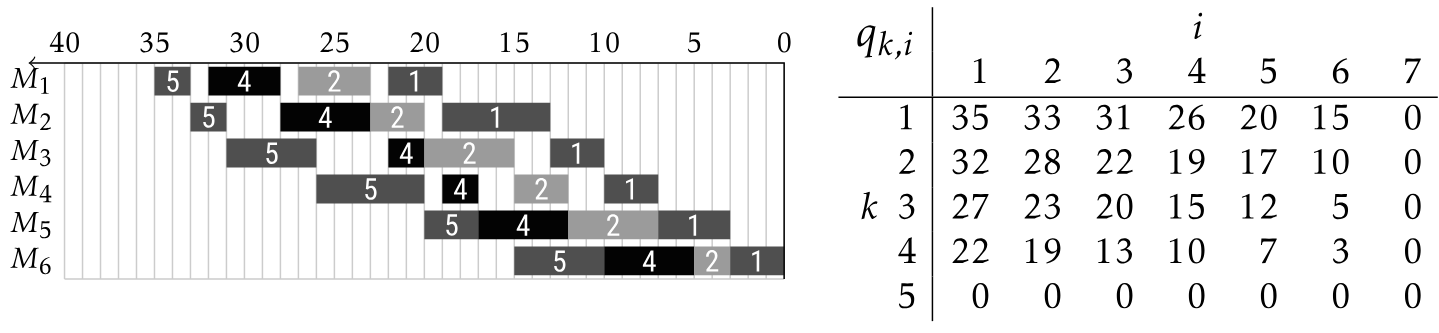
\includegraphics[width=0.8\textwidth]{
        ./.github/1733417731.png
      }
      \caption{Matriz de tiempos de iniciación 
      más tardios}\label{fig:Relative-latest-starting-times's-matrice}
    \end{figure}

    \textcolor{blue}{\textbf{Recuerda}: Los tiempo de inicio tardíos $q_{k, i}$ 
    después de la posición de inserción no cambian}

  \item Teniendo las dos matrices de tiempos de finalización más tempranos y los 
    tiempos de iniciación más tardios, calculamos la suma matricial (celda a 
    celda) de estos. \textcolor{blue}{Luego calculamos el máximo valor posible de 
    cada fila (comparamos sus columnas correspodientes), el valor resultante nos 
    indica el \textit{Makespan} de insertar el nuevo trabajo en dicha posición}

    \[
      \pi_0 = (J_4, J_5, J_1, J_2, \textcolor{red}{J_3}, J_6) \qquad 
      \pi = (J_5,J_4, J_2, J_1) \qquad \text{Next work:} J_3 
    \]

    \[
      \text{Calcule}\; MC_k = 
      \max_{i \in [m]}(e^{'}_{k, i} + q_{k, i}) \qquad
      \text{para}\; k \in [|\pi|+1]
    \]

    \begin{figure}[H]
      \centering
      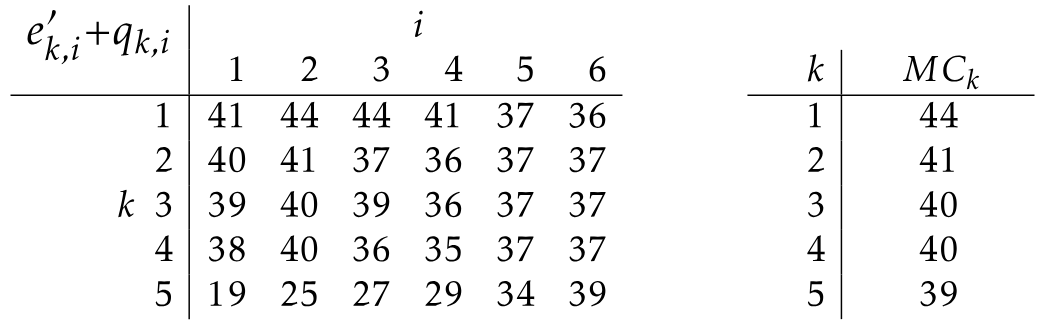
\includegraphics[width=0.8\textwidth]{
        ./.github/1733417752.png
      }
      \caption{Suma de las matrices y el mayor valor de 
      cada fila}\label{fig:sum-of-the-matrices-and-each-row's-value-max}
    \end{figure}

    \textcolor{blue}{Seleccionamos la posición de inserción con el minimo 
    \textit{Makespan}}
\end{enumerate}

Podemos verlo de forma gráfica para poder captar la idea de Taillard

\begin{figure}[H]
  \centering
  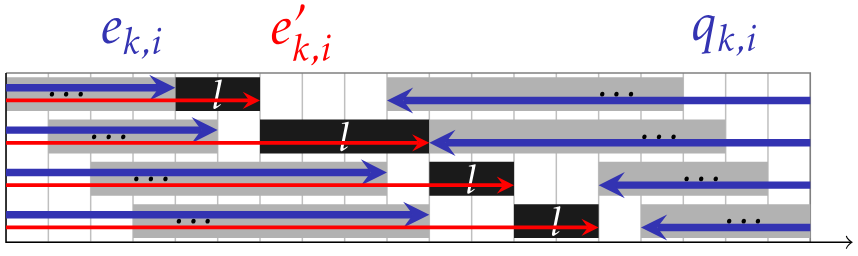
\includegraphics[width=0.8\textwidth]{./.github/1733417773.png}
  \caption{Resumen de los cálculos 
  realizados}\label{fig:overview-of-the-calculates-performed}
\end{figure}

Estos cáculos evaluan $n$ posiciones de inserción en un tiempo $O(nm)$. Con 
esta acelearción, NEH inserta los $n$ trabajos en un tiempo $O(n^2 m)$

\paragraph{Cuánto cueta la Heurística constructiva NEH}

Con esta aceleración, NEH inserta los $n$ trabajos en un tiempo $0(n^2 m)$

\begin{figure}[H]
  \centering
  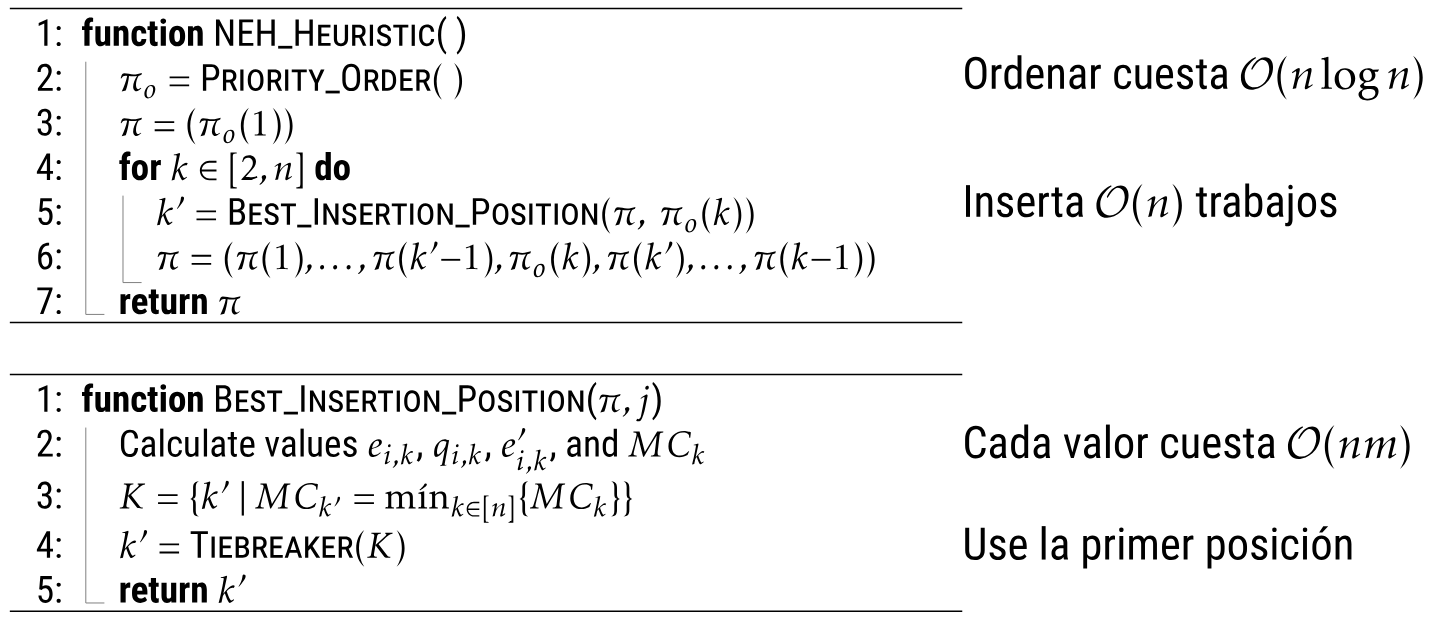
\includegraphics[width=0.8\textwidth]{./.github/1733417790.png}
  \caption{Complejidad temporal}\label{fig:time-complexity}
\end{figure}

\subsection{Heurísticas de búsqueda local}\label{sec:local-search-heuristic}

Comienzan desde una solución inicial (puede ser aleatoria), intentan reemplazar 
la solución actual por una mejor solución vecina, repiten este paso hasta que 
no hayan mejores soluciones vecinas. La pregunta que que ayuda a diseñar 
correctamente la Heurística es \textcolor{blue}{¿Qué cambio podría mejorar 
esta solución?}


\subsubsection{Que es la vecindad}

Es un subcconjunto del conjunto toal y le asigna a S dicho conjunto

\section{Metaheurísticas iterativas}\label{sec:iterative-heuristics}

\subsection{Búsqueda local iterativa (ILS)}\label{sec:iterative-lineal-search}

\subsection{Algoritmo iterativo goloso (IG)}\label{sec:greedy-iterative-algorithm}


\section{Preguntas y observaciones}\label{sec:questions-and-obsertation}

\begin{itemize}
  \item Acerca de la evaluación de la \textbf{Heurística constructiva}, 
    supuestamente el resultado tenemos que compararlo con el rendimiento 
    óptimo, ¿cómo podemos saber el óptimo si estamos en busca de ello?

  \item Acerca de la evaluación de la \textbf{Aceleración de Taillard} 
    \begin{enumerate}
      \item Cuando calculamos los tiempo de finalización más tempranos, ¿se realiza 
        para cada posición posible de inserción? Si es asi, en el ejemplo 
        se observa los resultados cuando se ha insertado al comienzo de todos 
        los trabajos \textcolor{blue}{¿Por qué cuando el nuevo trabajo lo inserto 
        en la primera posición, ya se calcula los tiempos de finalización si lo 
        inserto en las otras posiciónes?} Una posible respuesta es que los tiempos 
        de finalización más tempranos \textbf{antes de la posición de inserción 
        no cambian}

      \item Por qué se calcula el máximo tiempo de cada máquina y dicho valor 
        será donde se inserte el nuevo trabajo
    \end{enumerate}

  \item Acerca de la \textbf{Busqueda local}
    \begin{enumerate}
      \item Cuando yo saco el trabajo y lo inserto calculando el mejor 
        \textit{Makespan} (usando la acelearción de Taillard) ¿estoy realizando 
        teoricamente la inserción del minimo local de la vecindad actual (es 
        decir, el orden de los trabajos con la inserción hecha)?

      \item Por qué al realizar todas las inserciones posibles, tengo como 
        resultado solo un óptimo local y no un óptimo global
    \end{enumerate}
\end{itemize}

\section{Referencias}\label{sec:references}

\begin{itemize}
  \item Dr. Alexander Benavides
\end{itemize}

\end{document}
